%!TEX root = ../../../../report.tex

\subsection{Finite Element Method (FEM)} % (fold)
\label{sub:finite_element_method}
In the sections \ref{sub:limb_profile} and \ref{sub:rods}, pure mathematical tools have been used to calculate deformations and stresses.
This has been possible due to the simplification of the problem and the simple geometries found.
However, other parts have been analyzed with Finite Element Analysis (FEM), in which the part is subdivided into small volumes and then analyzed individually.
This allows the deformation and stress studies of complex geometries.

As an example, in the figures \ref{fig:fem_foot_iteration_1} and \ref{fig:fem_foot_iteration_2}, the iterative foot design is depicted.
Once the first iteration of the foot was modeled, the design has been changed in order to satisfy a minimum deformation criteria.
However, the designs have always been tested experimentally due to this analysis are under the assumption of isomorphic materials which, in the case of 3D printed parts like the shown in the figures, is not true.
The FEM studies have been used more as a qualitative analysis rather than quantitative.

\begin{figure}[ht]
    \centering
    \begin{subfigure}[b]{0.49\textwidth}
        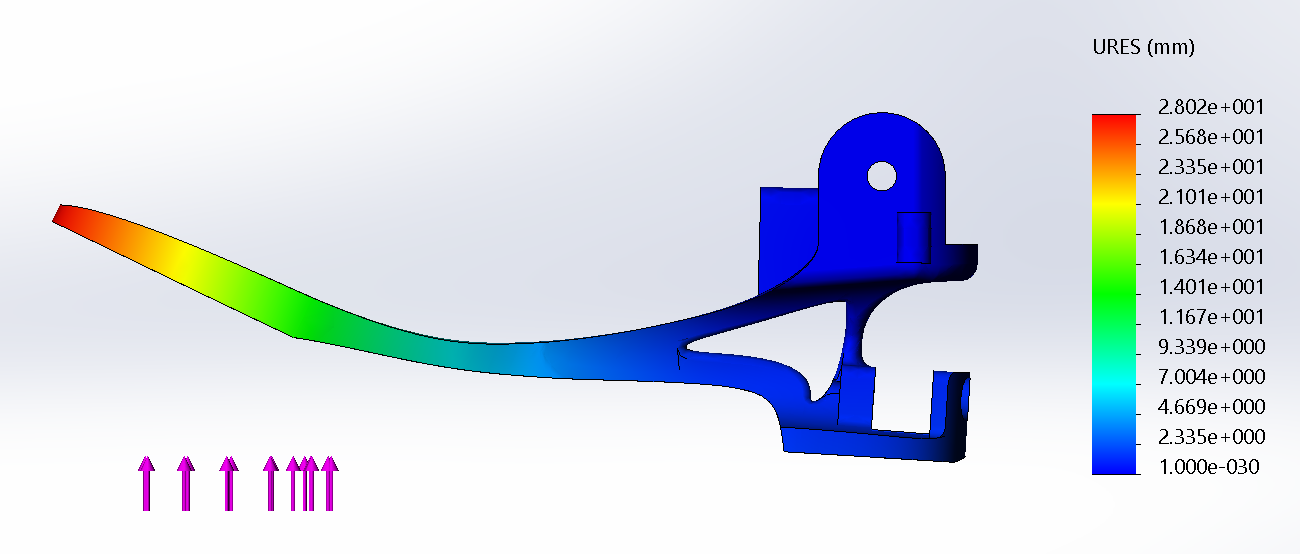
\includegraphics[width=\textwidth]{figures/fem_5N_1.PNG}
        \caption{FEM analysis in left foot iteration 1}
        \label{fig:fem_foot_iteration_1}
    \end{subfigure}
    \begin{subfigure}[b]{0.49\textwidth}
        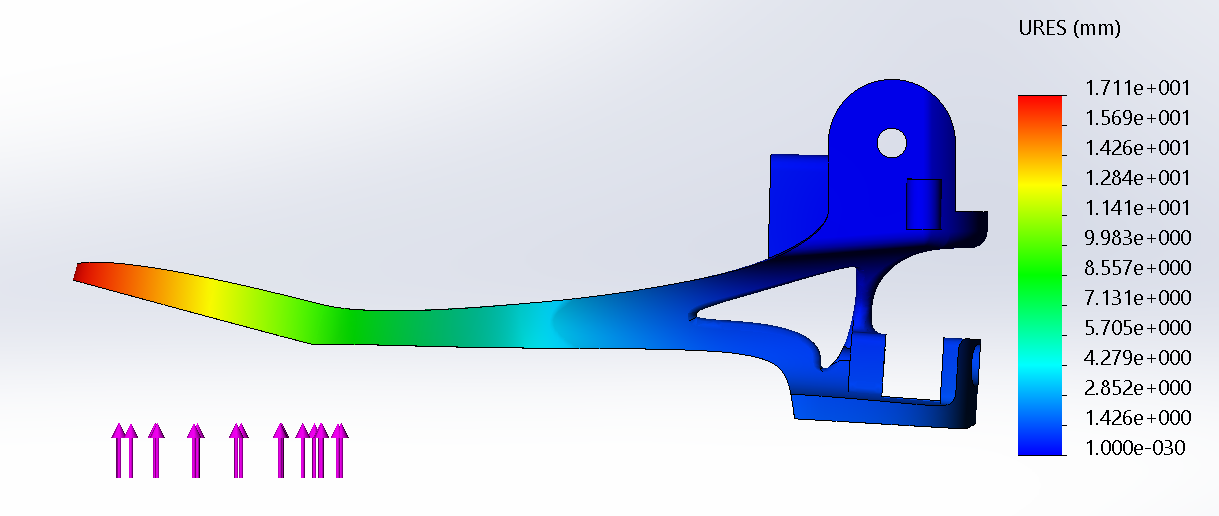
\includegraphics[width=\textwidth]{figures/fem_5N_2.PNG}
        \caption{FEM analysis in left foot iteration 2}
        \label{fig:fem_foot_iteration_2}
    \end{subfigure}
\end{figure}

% subsection finite_element_method (end)